\documentclass{article}
\usepackage[margin=1in]{geometry}
\usepackage[nodisplayskipstretch]{setspace}
\usepackage{amsmath, nccmath, bm}
\usepackage{amssymb}
\usepackage{enumitem}
\usepackage{graphicx}
\usepackage{float}
\usepackage{listings}
\usepackage{hyperref}
\usepackage[svgnames]{xcolor}
\usepackage{indentfirst}
%\usepackage{chngcntr}
%\counterwithin{table}{section}
\graphicspath{
{./images}}

%\hypersetup{
%    colorlinks=true,
%    linkcolor=black,
%    filecolor=black,      
%    urlcolor=blue
%    }

\newcommand{\zerodisplayskip}{
	\setlength{\abovedisplayskip}{0pt}%
	\setlength{\belowdisplayskip}{0pt}%
	\setlength{\abovedisplayshortskip}{0pt}%
	\setlength{\belowdisplayshortskip}{0pt}%
	\setlength{\mathindent}{0pt}}
	
\definecolor{vgreen}{RGB}{104,180,104}
\definecolor{vblue}{RGB}{49,49,255}
\definecolor{vorange}{RGB}{255,143,102}

\lstdefinestyle{verilog-style}
{
    language=Verilog,
    basicstyle=\small\ttfamily,
    keywordstyle=\color{vblue},
    identifierstyle=\color{black},
    commentstyle=\color{vgreen},
    numbers=left,
    numberstyle=\tiny\color{black},
    numbersep=10pt,
    tabsize=8,
    moredelim=*[s][\colorIndex]{[}{]},
    literate=*{:}{:}1
}

\lstset{style={verilog-style},showstringspaces=false}

\lstdefinestyle{nocoloring}{
    keywordstyle=\color{black},
    commentstyle=\color{black},
    stringstyle=\color{black}
}

\makeatletter
\newcommand*\@lbracket{[}
\newcommand*\@rbracket{]}
\newcommand*\@colon{:}
\newcommand*\colorIndex{%
    \edef\@temp{\the\lst@token}%
    \ifx\@temp\@lbracket \color{black}%
    \else\ifx\@temp\@rbracket \color{black}%
    \else\ifx\@temp\@colon \color{black}%
    \else \color{vorange}%
    \fi\fi\fi
}
\makeatother

\newcommand{\code}[1]{%
	\colorbox{Gainsboro}{\texttt{#1}}%
}

\title{Lab 3}
\author{Owen Sowatzke}
\date{April 21, 2025}

\begin{document}

	% \offinterlineskip
	% \setlength{\lineskip}{12pt}
	% \zerodisplayskip
	\maketitle
	
	\section{Introduction}
	
	In this lab, we perform design and verification for an ARM 8-bit microprocessor. We start by simulating a SystemVerilog model of the microprocessor in NC verilog. Then, we design 8-bit AND and OR wordslices in Cadence Virtuoso. For each of these wordslices, we create a schematic, symbol, and layout. Then, we incorporate each of our wordslices into the ALU schematic and layout. Similarly, we update the datapath layout with our updated ALU. At each stage of the design, we verify our layouts using DRC and LVS. Finally, we create a netlist from our design and validate its behavior in simulation. 
	
	\section{SystemVerilog Model RTL Simulation}
	
	In this section, we intended to show the results of our NC-Verilog  simulation. However, there was an IT issue on the session server that prevented us from running NC-Verilog. When, we tried the command provided in the lab description, we obtained the following results:
	
	\begin{figure}[H]
		\centerline{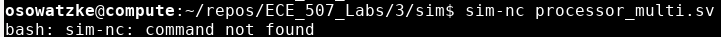
\includegraphics[width=0.8\textwidth]{sim_error.png}}
		\caption{Simulation Error When Attempting to Run NC Verilog}
		\label{fig::sim_error}
	\end{figure}
	 
	\section{AND Wordslice}
	\label{section::and_wordslice}
	
	In this section, we perform design and verification of our AND wordslice. Our wordslice specifically contains 8 \texttt{and2\_1x} gates from the \texttt{muddlib11} library. The resulting schematic is shown in Figure \ref{fig::and2_1x_8_schematic}. Note the vectorized ports and component instances.
	
	\begin{figure}[H]
		\centerline{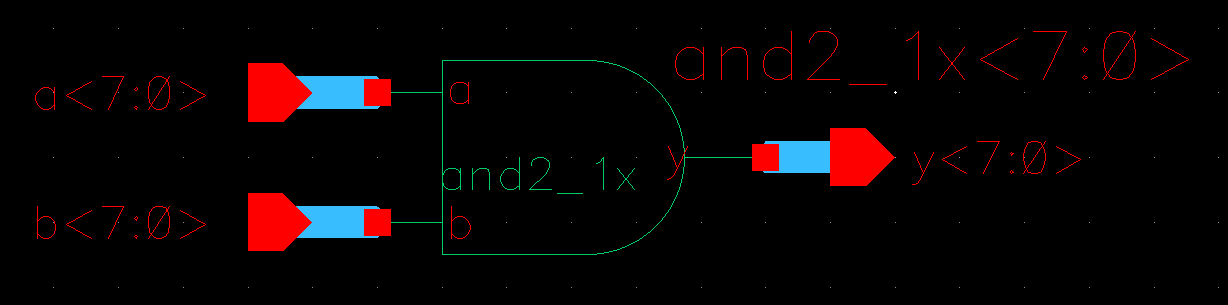
\includegraphics[width=0.5\textwidth]{and2_1x_8_schematic.png}}
		\caption{Schematic for AND Wordslice}
		\label{fig::and2_1x_8_schematic}
	\end{figure}
	
	\noindent Next, we create a symbol for our AND wordslice. For this step, we start with a copy of the \texttt{and2\_1x} symbol and make small incremental updates. Our wordslice symbol with these updates is shown in Figure \ref{fig::and2_1x_8_symbol}. Note that the port names and wire widths have been updated to reflect the vectorized inputs and outputs.
	
	\begin{figure}[H]
		\centerline{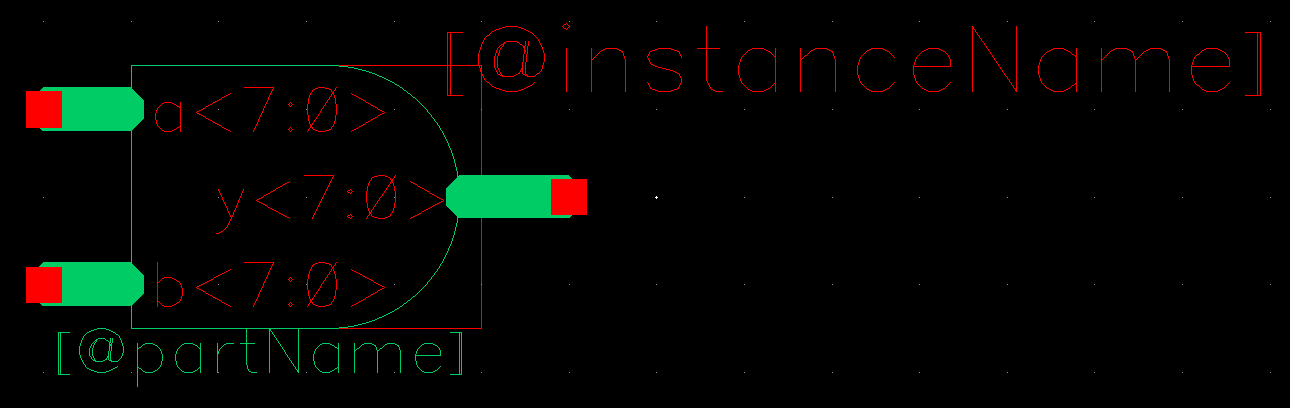
\includegraphics[width=0.5\textwidth]{and2_1x_8_symbol.png}}
		\caption{Symbol for AND Wordslice}
		\label{fig::and2_1x_8_symbol}
	\end{figure}
	
	\noindent Then, we create a layout for our wordslice. For the layout, we use an $8 \times 1$ mosiac of AND gates. The resulting layout with different display levels is shown in Figures \ref{fig::and2_1x_8_layout_mosiac_overview} and \ref{fig::and2_1x_8_layout_detailed}. Note that the our images are rotated $90^{\circ}$ with respect to the layouts.  
	
	\begin{figure}[H]
		\centerline{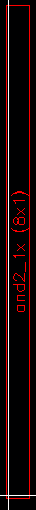
\includegraphics[height=0.8\textwidth, angle=270]{and2_1x_8_layout_mosiac_overview.png}}
		\caption{AND Gate Mosiac Layout Display Level = 0}
		\label{fig::and2_1x_8_layout_mosiac_overview}
	\end{figure}
	
	\begin{figure}[H]
		\centerline{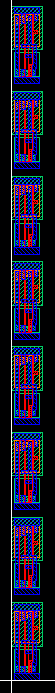
\includegraphics[height=0.8\textwidth, angle=270]{and2_1x_8_layout_detailed.png}}
		\caption{AND Gate Mosiac Layout Display Level = 1}
		\label{fig::and2_1x_8_layout_detailed}
	\end{figure}
	
	\noindent After placing the AND gates, we placed input and output ports for each gate. However, virtuoso shorted each element of the input/output buses. These shorts are displayed on an individual AND gates in Figure \ref{fig::and2_1x_8_cell_with_shorts} and in the Annotation Browser in Figure \ref{fig::and2_1x_8_annotation_shorts}. 
	
	\begin{figure}[H]
		\centerline{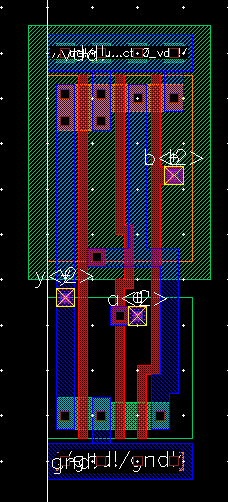
\includegraphics[width=0.2\textwidth]{and2_1x_8_cell_with_shorts.png}}
		\caption{Shorts Marked in the Schematic}
		\label{fig::and2_1x_8_cell_with_shorts}
	\end{figure}
	
	\begin{figure}[H]
		\centerline{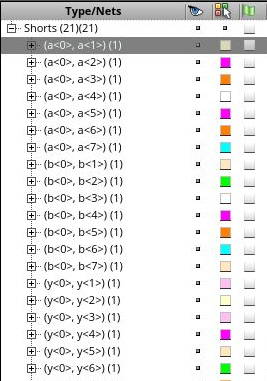
\includegraphics[width=0.35\textwidth]{and2_1x_8_annotation_shorts.png}}
		\caption{Shorts Called Out by the Annotation Browser}
		\label{fig::and2_1x_8_annotation_shorts}
	\end{figure}
	
	\noindent To work around this, I instantiated a single AND gate and then copied it 7 times with $33{\mu}m$ spacing. The resulting schematic at display level = 0 is shown in Figure \ref{fig::and2_1x_8_layout_overview}. Note that the AND gates are now displayed individually at this display level. However, the underlying content is the same.
	
	\begin{figure}[H]
		\centerline{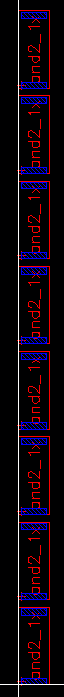
\includegraphics[height=0.8\textwidth, angle=270]{and2_1x_8_layout_overview.png}}
		\caption{AND Wordslice Created without Mosiac at Display Level = 0}
		\label{fig::and2_1x_8_layout_overview}
	\end{figure}
	
	\noindent For better visualization, we also highlight the port placement for a single AND gate, which is shown in Figure \ref{fig::and2_1x_8_single_gate_ports}.
	
	\begin{figure}[H]
		\centerline{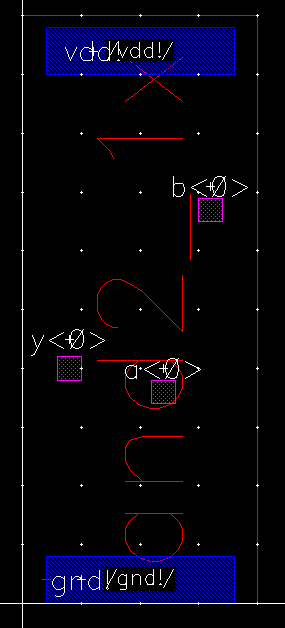
\includegraphics[width=0.25\textwidth]{and2_1x_8_single_gate_ports.png}}
		\caption{Port Placement for a Given AND Gate}
		\label{fig::and2_1x_8_single_gate_ports}
	\end{figure}
	
	\noindent Next, we performed DRC and LVS for our layout. According to the Cadence Virtuoso IC23.1 documentation, we should have been able to do this with Verify \textgreater\ DRC and Verify \textgreater\ LVS. However, the Verify drop-down menu did not include these options. The drop-down menu from our Virtuoso installation is shown in Figure \ref{fig::verify_dropdown_menu}, and the expected menu is shown in Figure \ref{fig::verify_dropdown_menu_doc}.
	
	\begin{figure}[H]
		\centerline{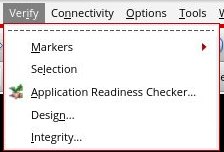
\includegraphics[width=0.4\textwidth]{verify_dropdown_menu.png}}
		\caption{Verify Drop-Down Menu in Layout Window}
		\label{fig::verify_dropdown_menu}
	\end{figure}
	
	\begin{figure}[H]
		\centerline{\fbox{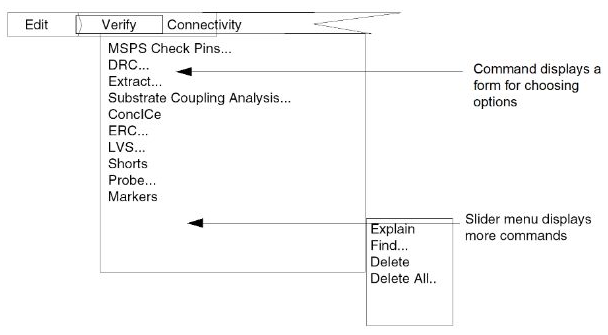
\includegraphics[height=0.4\textwidth]{verify_dropdown_menu_doc.png}}}
		\caption{Verify Drop-Down Menu per Documentation}
		\label{fig::verify_dropdown_menu_doc}
	\end{figure}
	
	\noindent Luckily, we were able to perform comparable analysis using Verify \textgreater\ Design... and Verify \textgreater\ Application Readiness Checker.... However, neither of these dropdowns included the "Join Nets with the Same Name" option given in the lab manual. Instead, I had to create "Must Connect" groups for gnd! and vdd! using Pins \textgreater\ Pin Connectivity Setting.... Additionally, I had to associate each of the AND gates in the schematic with gates in my layout using Connectivity \textgreater\ Define Device Correspondence. After performing these updates, I was able to generate the DRC and LVS results shown in Figures \ref{fig::and_drc} and \ref{fig::and_lvs} respectively.
	
	\begin{figure}[H]
		\centerline{\fbox{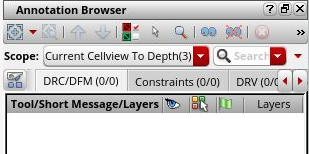
\includegraphics[width=0.5\textwidth]{and_drc.png}}}
		\caption{DRC Annotations Showing All Checks Passing}
		\label{fig::and_drc}
	\end{figure}
	
	\begin{figure}[H]
		\centerline{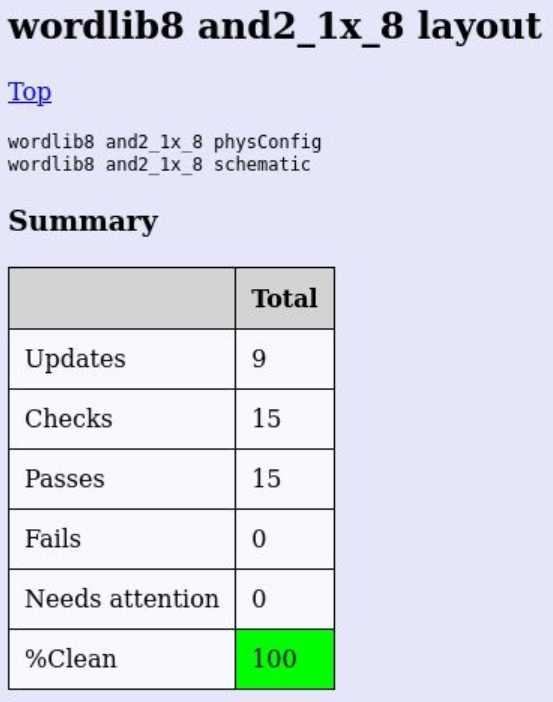
\includegraphics[width=0.4\textwidth]{and_lvs.png}}
		\caption{Passing LVS Checks}
		\label{fig::and_lvs}
	\end{figure}
	
	\section{OR Wordslice}
	
	In this section, we repeat the process given in Section \ref{section::and_wordslice} to create an OR wordslice.  Our wordslice specifically contains 8 \texttt{or2\_1x} gates from the \texttt{muddlib11} library. The resulting schematic is shown in Figure \ref{fig::or2_1x_8_schematic}. Note the vectorized ports and component instances.
	
	\begin{figure}[H]
		\centerline{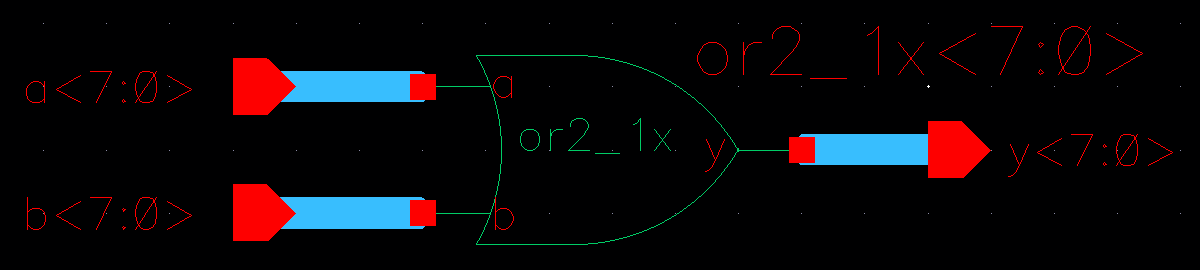
\includegraphics[width=0.5\textwidth]{or2_1x_8_schematic.png}}
		\caption{Schematic for OR Wordslice}
		\label{fig::or2_1x_8_schematic}
	\end{figure}
	
	\noindent Next, we create a symbol for our OR wordslice. For this step, we start with a copy of the \texttt{or2\_1x} symbol and make small incremental updates. Our wordslice symbol with these updates is shown in Figure \ref{fig::or2_1x_8_symbol}. Note that the port names and wire widths have been updated to reflect the vectorized inputs and outputs.
	
	\begin{figure}[H]
		\centerline{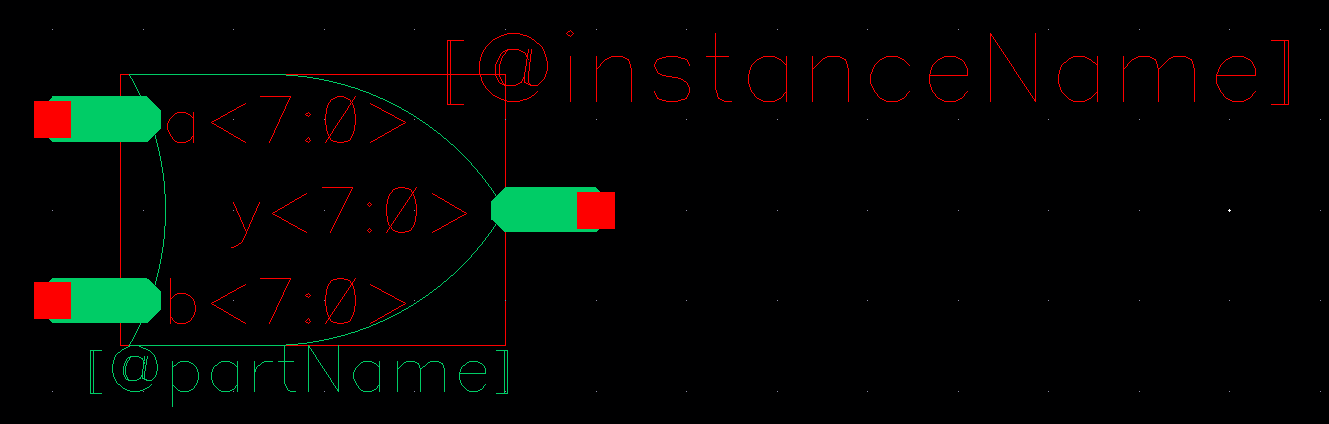
\includegraphics[width=0.5\textwidth]{or2_1x_8_symbol.png}}
		\caption{Symbol for OR Wordslice}
		\label{fig::or2_1x_8_symbol}
	\end{figure}
	
	\noindent Then, we create a layout for our wordslice. We leverage what we learned from the previous section and copy OR gates instead of using a mosiac. This prevents us from creating unintentional shorts. The layout with different display levels is shown in Figures \ref{fig::or2_1x_8_layout_overview} and \ref{fig::or2_1x_8_layout_detailed}.
	
	\begin{figure}[H]
		\centerline{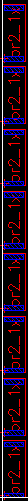
\includegraphics[height=0.8\textwidth, angle=270]{or2_1x_8_layout_overview.png}}
		\caption{OR Wordslice Layout Display Level = 0}
		\label{fig::or2_1x_8_layout_overview}
	\end{figure}
	
	\begin{figure}[H]
		\centerline{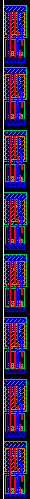
\includegraphics[height=0.8\textwidth, angle=270]{or2_1x_8_layout_detailed.png}}
		\caption{OR Wordslice Layout Display Level = 1}
		\label{fig::or2_1x_8_layout_detailed}
	\end{figure}
	
	\noindent We also highlight the port placement for a single OR gate, which is shown in Figure \ref{fig::or2_1x_8_single_gate_ports}.
	
	\begin{figure}[H]
		\centerline{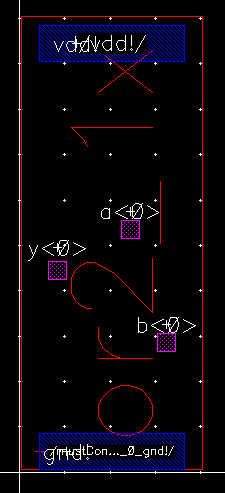
\includegraphics[width=0.25\textwidth]{or2_1x_8_single_gate_ports.png}}
		\caption{Port Placement for a Given OR Gate}
		\label{fig::or2_1x_8_single_gate_ports}
	\end{figure}
	
	\noindent Finally, following the procedure from the previous section, we perform DRC and LVS checks. To avoid LVS errors, we map gates in the schematic to gates in the layout and create "Must Connect" groups for gnd! and vdd! The DRC and LVS results are shown in Figures \ref{fig::or_drc} and \ref{fig::or_lvs} respectively.
	
	\begin{figure}[H]
		\centerline{\fbox{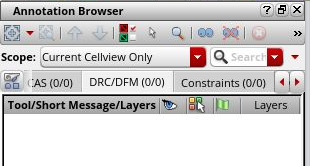
\includegraphics[width=0.5\textwidth]{or_drc.png}}}
		\caption{DRC Annotations Showing All Checks Passing}
		\label{fig::or_drc}
	\end{figure}
	
	\begin{figure}[H]
		\centerline{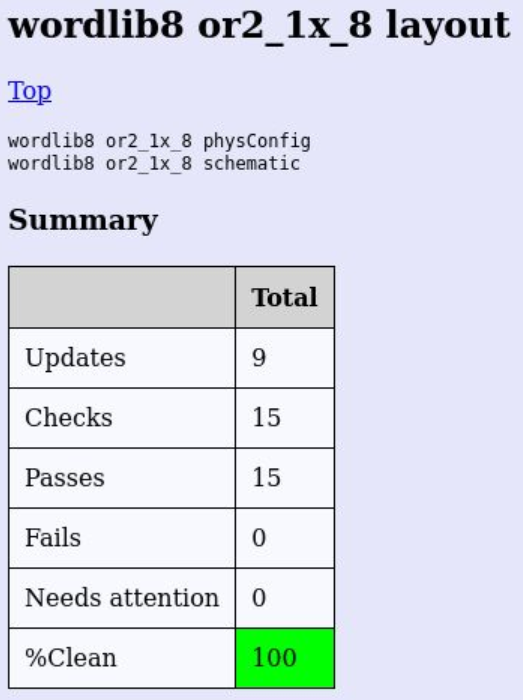
\includegraphics[width=0.4\textwidth]{or_lvs.png}}
		\caption{Passing LVS Checks}
		\label{fig::or_lvs}
	\end{figure}
	
	\section{ALU}
	
	In this section, we complete the ALU schematic using the AND and OR wordslices we created in the previous sections. The resulting schematic is shown in Figure \ref{fig::alu_schematic}.
	
	\begin{figure}[H]
		\centerline{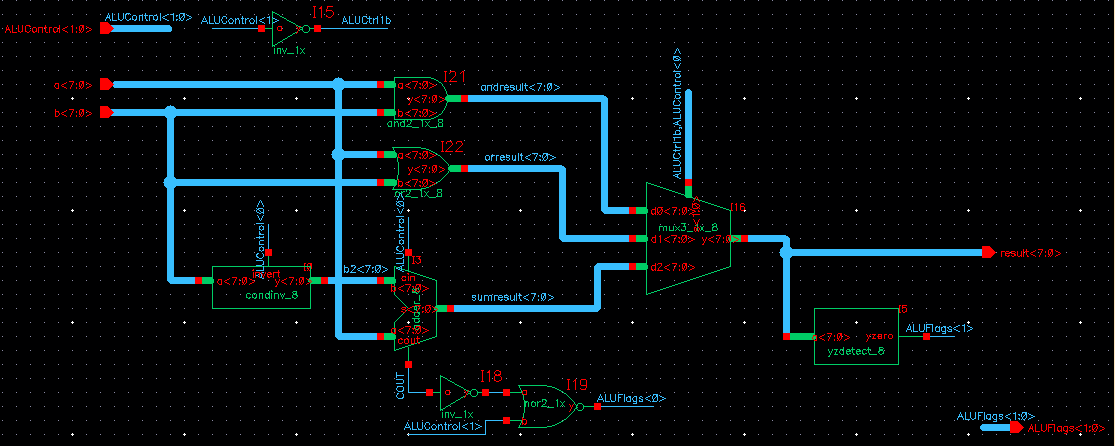
\includegraphics[width=0.9\textwidth]{alu_schematic.png}}
		\caption{ALU Schematic after Adding AND and OR Wordslices}
		\label{fig::alu_schematic}
	\end{figure}
	
	\noindent Then, we modify the ALU layout to include the AND and OR wordslices. The layout with different display levels is shown in Figures \ref{fig::alu_layout_overview} and \ref{fig::alu_layout_detailed}. Note that the our figures are rotated $90^{\circ}$ with respect to the layouts. The AND wordslice (top) and OR wordslice (bottom) are highlighted in our figure.
	
	\begin{figure}[H]
		\centerline{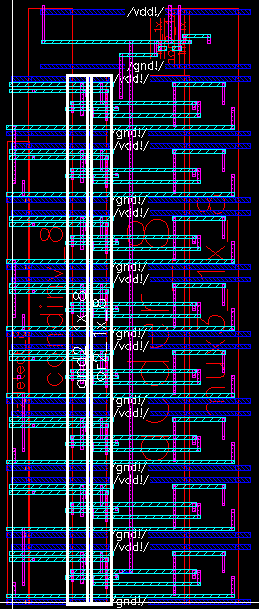
\includegraphics[height=0.8\textwidth, angle=270]{alu_layout_overview.png}}
		\caption{ALU Layout Display Level = 0}
		\label{fig::alu_layout_overview}
	\end{figure}
	
	\begin{figure}[H]
		\centerline{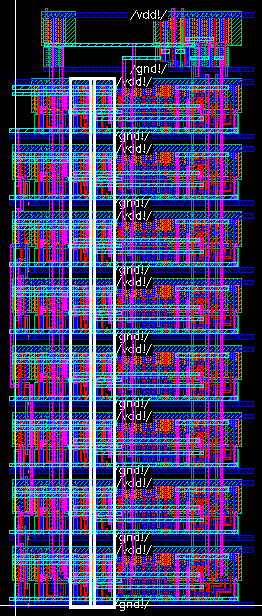
\includegraphics[height=0.8\textwidth, angle=270]{alu_layout_detailed.png}}
		\caption{ALU Layout Display Level = 1}
		\label{fig::alu_layout_detailed}
	\end{figure}
	
	% \noindent We focus on the layout for the first bit of the ALU datapath in Figure \ref{fig::alu_layout_bit0}. The AND and OR wordslices are highlighted in the figure. The AND wordslice is on the left, and the OR wordslice is on the right. Examining the layout, we see that the inputs of both gates are correctly connected to the \texttt{a} and \texttt{b} bitlines. Additionally, we see that the output of the AND gate is connected to \texttt{d0}, while the output of the OR gate is connected to \texttt{d1}. This is consistent with our schematic shown in Figure \ref{fig::alu_schematic}.
	
	\begin{figure}[H]
		\centerline{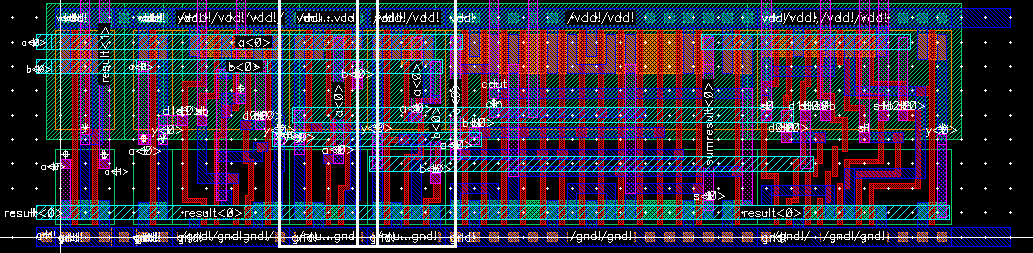
\includegraphics[width=0.8\textwidth]{alu_layout_bit0.png}}
		\caption{Layout for the First Bit of the ALU Datapath}
		\label{fig::alu_layout_bit0}
	\end{figure}
	
	\noindent Finally, after properly associating the components in the schematic to the components in the layout, we perform DRC and LVS checks for our layout. The results are included in Figures \ref{fig::alu_drc} and \ref{fig::alu_lvs} respectively.
	
	\begin{figure}[H]
		\centerline{\fbox{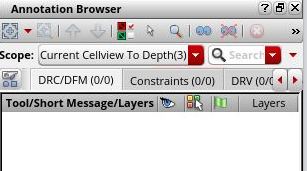
\includegraphics[width=0.5\textwidth]{alu_drc.png}}}
		\caption{DRC Annotations Showing All Checks Passing}
		\label{fig::alu_drc}
	\end{figure}
	
	\begin{figure}[H]
		\centerline{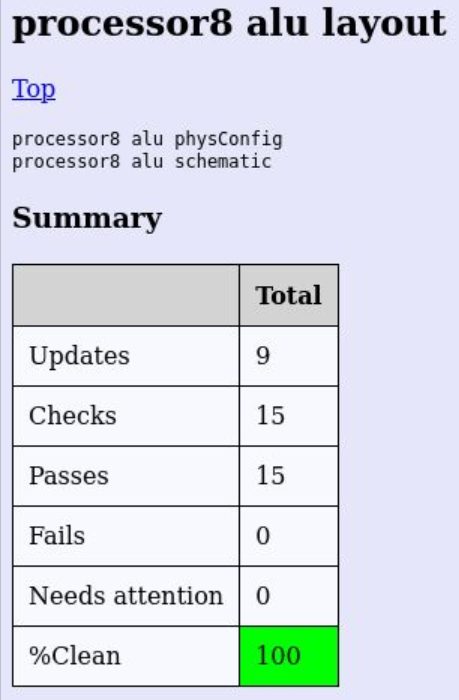
\includegraphics[width=0.4\textwidth]{alu_lvs.png}}
		\caption{Passing LVS Checks}
		\label{fig::alu_lvs}
	\end{figure}
	
	\section{Datapath}
	
	In this section, we perform DRC and LVS checks for the datapath schematic with the updated ALU. We also show the schematic for the datapath in Figure \ref{fig::datapath_schematic}. Note that we do not need to make any edits to the schematic because the ALU block is already included and its ports are unchanged.
	
	\begin{figure}[H]
		\centerline{\fbox{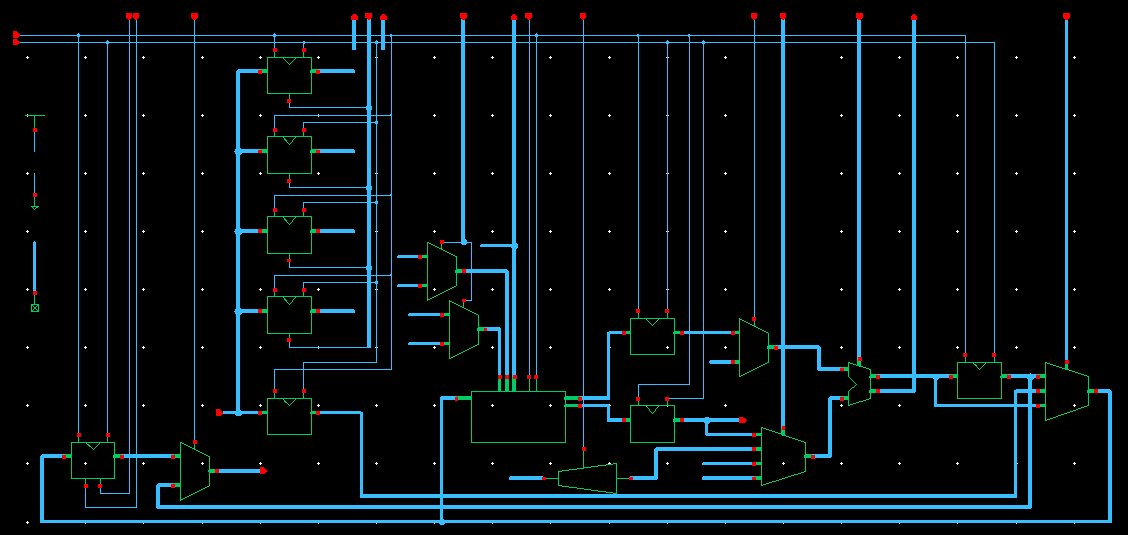
\includegraphics[width=0.9\textwidth]{datapath_schematic.png}}}
		\caption{Datapath Schematic}
		\label{fig::datapath_schematic}
	\end{figure}
	
	\noindent Next, we show the layout of the datapath in Figure \ref{fig::datapath_layout}.
	
	\begin{figure}[H]
		\centerline{\fbox{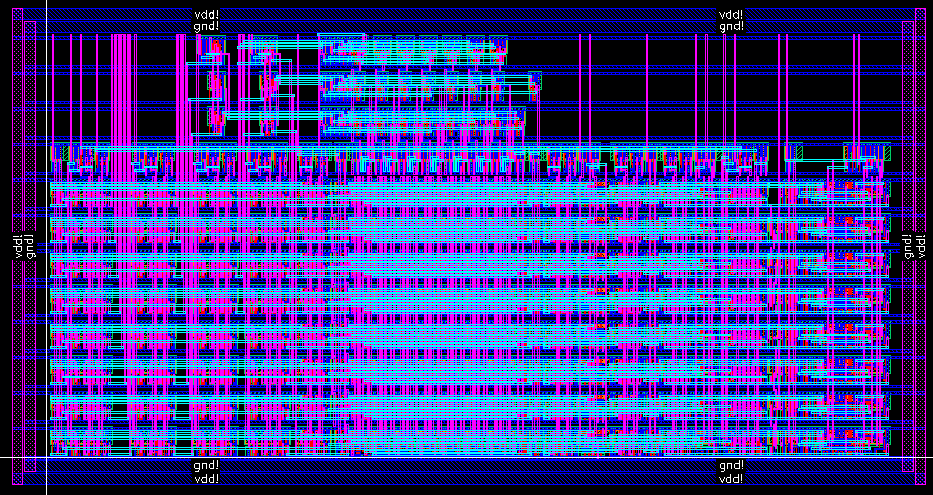
\includegraphics[width=0.9\textwidth]{datapath_layout.png}}}
		\caption{Datapath Layout}
		\label{fig::datapath_layout}
	\end{figure}
	
	\noindent Note that layout automatically pulls the updates from the ALU layout. However, we still need to perform DRC and LVS checks to validate the overall design. Our DRC and LVS results after mapping blocks in our layout to blocks in our schematic are shown in Figures \ref{fig::datapath_drc} and \ref{fig::datapath_lvs} respectively.
	
	\begin{figure}[H]
		\centerline{\fbox{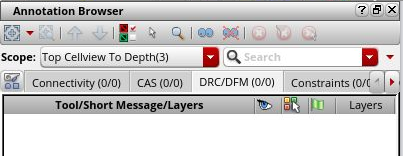
\includegraphics[width=0.5\textwidth]{datapath_drc.png}}}
		\caption{DRC Annotations Showing All Checks Passing}
		\label{fig::datapath_drc}
	\end{figure}
	
	\begin{figure}[H]
		\centerline{\fbox{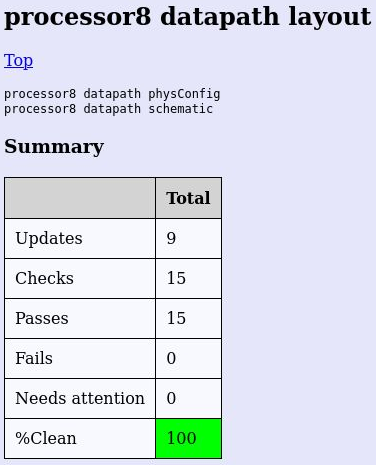
\includegraphics[width=0.4\textwidth]{datapath_lvs.png}}}
		\caption{Passing LVS Checks}
		\label{fig::datapath_lvs}
	\end{figure}
	
	\section{Datapath Simulation}
	
	In this section, we attempt to generate a netlist from our datapath and simulate it. First, to generate the netlist we go to Launch \textgreater\ Plugins \textgreater\ Simulation \textgreater\ NC-Verilog. This opened the following window:
	
	\begin{figure}[H]
		\centerline{\fbox{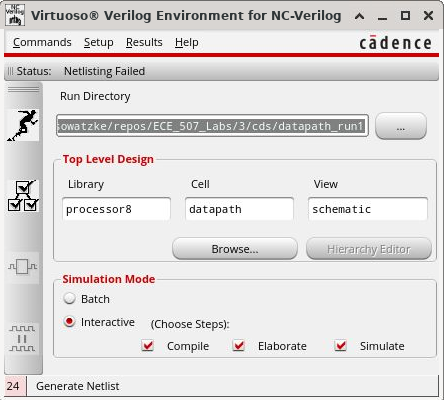
\includegraphics[width=0.5\textwidth]{nc_verilog_sim.png}}}
		\caption{NC-Verilog Simulation Window}
		\label{fig::nc_verilog_sim}
	\end{figure}
	
	\noindent Using the window, we attempted to generate a netlist for our design. However, we received errors in the generation process, which are illustrated in Figure \ref{fig::netlist_generation_errors}.
	
	\begin{figure}[H]
		\centerline{\fbox{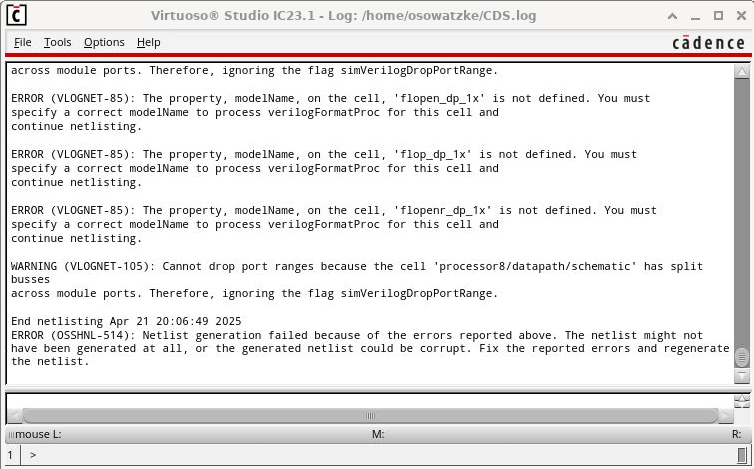
\includegraphics[width=0.5\textwidth]{netlist_generation_errors.png}}}
		\caption{Netlist Generation Errors}
		\label{fig::netlist_generation_errors}
	\end{figure}
	
	\noindent Interestingly, none of the errors occurred in modules that we modified, indicating a potential source file error or tool error. Because of these errors, we were unable to generate a netlist and perform a simulation. However, we still learned the procedure for generating a netlist, which we could use in simulation to verify our design.
	
	\section{Conclusion}
	
	In this lab, we performed design and verification for an ARM 8-bit microprocessor. We attempted to simulate a SystemVerilog model of the microprocessor in NC verilog. However, due to an IT issue on the session server, we were unable to perform this simulation. We also designed 8-bit AND and OR wordslices in Cadence Virtuoso. For each of these wordslices, we created a schematic, symbol, and layout. While creating the layout, we ran into problem with the mosiac command creating uintentional short circuits. We were able to work around this by creating multiple copies of the same cell. 
	
	Next, we performed DRC and LVS for our layouts. To resolve the errors we found, we had to perform two actions. First, we had to associate gates in our layout with gates in our schematic. Then, we had to create "Must Connect" groups for gnd! and vdd! After these steps were complete, we received passing DRC and LVS results. 
	
	Once our wordslices were validated, we incorporated them into the ALU schematic and layout. Then, we performed DRC and LVS on our layout. After applying lessons learned from the AND/OR wordslice layouts, we received passing DRC and LVS results. After validating our layout, we performed DRC and LVS on the datapath in a similar fashion and received passing results. Finally, we attempted to generate a netlist from the datapath schematic. Unfortunately, another source file and/or IT issue prevented us from fully generating the netlist. Even though we were unable to generate the netlist, we still learned how to use the tools and how to validate our designs.
	
\end{document}